% % \part{优化模型}
% % \chapter{线性规划和整数规划}

% \documentclass[UTF8]{ctexbook}

% \ctexset{
%     part/number = \chinese{part}
% }
% \usepackage{amsmath}% ams 数学公式
% \usepackage{mathtools}% ams 数学公式
% \usepackage{amsfonts}% ams 数学字体
% \usepackage{amssymb,latexsym}% ams 数学符号与LaTeX数学符号
% \usepackage{mathrsfs}% 花式符号
% \usepackage{ntheorem}%定理、定义、证明
%   \theoremstyle{nonumberplain}
%   \theoremheaderfont{\bfseries}
%   \theorembodyfont{\normalfont}
%   \theoremsymbol{$\square$}
%   \newtheorem{Proof}{\hskip 2em 证明}
%   \newtheorem{theorem}{\hspace{2em}定理}[chapter]
%   \newtheorem{definition}{\hspace{2em}定义}[chapter] % 如果没有章, 只有节, 把上面的[chapter]改成[section]
%   \newtheorem{axiom}[definition]{\hspace{2em}公理}
%   \newtheorem{lemma}[definition]{\hspace{2em}引理}
%   \newtheorem{proposition}[definition]{\hspace{2em}命题}
%   \newtheorem{corollary}[definition]{\hspace{2em}推论}
%   \newtheorem{remark}{\hspace{2em}注}[chapter] %类似地定义其他“题头”. 这里“注”的编号与定义、定理等是分开的

% \usepackage{enumerate}%itemiz环境。\begin{enumerate}[step 1]
% \usepackage{cite}%参考文献
%     \bibliographystyle{plain}
% \usepackage{extarrows}% 带参数的箭头
% \usepackage{hyperref}% 超链接
% %\usepackage[CJKbookmarks, colorlinks, bookmarksnumbered=true,pdfstartview=FitH,linkcolor=black,citecolor=black]{hyperref}%超链接的格式设置
% \hypersetup{
%     colorlinks=false,% 去掉超链接颜色
%     pdfborder=0 0 0% 取消超链接的边框
% }
% \usepackage{graphicx}% 图片管理
% \usepackage{caption}
% \usepackage{subcaption}%并排的图各有标题
% \graphicspath{{images/}}% 设置图片搜索路径
% \usepackage{float,varwidth}% 浮动体
% \usepackage{booktabs}% 三线表
% \usepackage{fancyhdr}% 页眉设置
% \usepackage{xcolor}% 颜色宏包
% \usepackage{colortbl}% 彩色表格
% \usepackage{listings}% 代码高亮
% \usepackage{caption}% 对标题进行控制,如让\caption标题的字体缩小一号,同时数字标签使用粗体可以用:\usepackage[font=small,labelfont=bf]{caption}
% \usepackage{xfrac,upgreek}%分别是行间公式如a/b的形式(将原来的命令\frac改成\sfrac)和希腊字体的宏包的
% \usepackage{mathtools}%lgathered和rgathered环境把公式向左向右对齐
% \usepackage{tabularx}%提供自动延伸的表列,(X列格式说明符),文字过长时可以自动转行
% \usepackage{longtable}%长表格
% \usepackage{enumitem}%enumerate宏包的升级
% \usepackage{harpoon}%数学公式的矢量
% \usepackage{bookmark}%目录的书签
% \usepackage{pifont}%给数字加上圈。然后在正文输入\ding{172}~\ding{211}得到相应数字,要是要①就输入:\ding{172}②就输:\ding{173}
% \renewcommand{\headwidth}{\textwidth}%图片并排,这个要列在所有宏包的后面
% \makeatletter
% \newcommand{\rmnum}[1]{\romannumeral #1}
% \newcommand{\Rmnum}[1]{\expandafter\@slowromancap\romannumeral #1@}
% \makeatother
% \definecolor{codegreen}{rgb}{0,0.6,0}
% \definecolor{codegray}{rgb}{0.5,0.5,0.5}
% \definecolor{codepurple}{rgb}{0.58,0,0.82}
% \definecolor{backcolour}{rgb}{0.95,0.95,0.92}
% \lstset{
%     commentstyle=\color{codegreen},
%     keywordstyle=\color{magenta},
%     numberstyle=\tiny\color{codegray},
%     stringstyle=\color{codepurple},
%     basicstyle=\footnotesize,
%     breakatwhitespace=false,% 断行只在空格处
%     breaklines=true,% 自动断行
%     captionpos=b,% 标题位置
%     keepspaces=true,
%     numbers=left,
%     numbersep=5pt,
%     showspaces=false,
%     showstringspaces=false,
%     showtabs=false,% 显示
%     tabsize=2% TAB 被当作两个空格
% }
% \topmargin=0pt\oddsidemargin=0pt\evensidemargin=0pt
% \textwidth=16.5cm\textheight=23cm\raggedbottom%我这么设置是为了缩小页边距,满足有的文字无法转行
% \pagestyle{headings}%页眉为章节标题,无页脚
% \setlength{\abovecaptionskip}{4pt}
% \setlength{\belowcaptionskip}{-8pt}%图片表格的前后距离设置
% \CTEXsetup[format={\zihao{-3}\raggedright\bfseries}]{section}%设置节的格式

% \begin{document}
% \part{优化模型}
\chapter{线性规划}

\section{问题的引入与分析}
    \par
    前面,我们讨论的都是非线性规划,无约束非线性规划和约束非线性规划,下面,我们讨论两种特殊情况:1.线性规划2.二次规划。线性规划要求目标函数和约束条件皆为线性函数。二次规划则要求目标函数为二次函数。我们先来讨论线性规划。
    \par
    示例:设某工厂用4种资源生产3种产品,单位$j$产品需要$i$资源的数量为$a_{ij}$,可获利$c_j$。并要求第$i$种资源总消耗不超过$b_i$,第$j$种产品产量不超过$d_j$,问如何安排生产使总利润最大?
    \par
    解:设3种产品的产量分别为$x_1,x_2,x_3$,则
    \begin{align*}
    &{\max}\ \mathop{\sum}\limits_{j=1}^3c_jx_j\\
    &s.t.\left\{
    \begin{aligned}
    &\mathop{\sum}\limits_{j=1}^3a_{ij}x_j \leqslant b_i\quad i=1,2,3,4\\
    &x_j \leqslant d_j\\
    &x_j \geqslant 0\\
    &j=1,2,3
    \end{aligned}
    \right.
    \end{align*}
    \par
    线性规划的目标函数$f$是线性的,约束函数是线性的,约束有等式和不等式两种。Optimization Toolbox采用下列3种方法求解线性规划:
    \par
    \ding{172}单纯形算法,也是最常用的算法;
    \par
    \ding{173}内点算法:基于原始预估校正算法,尤其适用于稀疏结构或其它特殊结构的大规模问题;
    \par
    \ding{174}动态序列算法。
\section{模型规范化及基本理论}
    \par
    线性规划的一般形式为
    \begin{align*}
    & \mathop{\min}\limits_{x\in R^n}\ f(x)=c^\mathrm{T} x\\
    &s.t.\left\{
    \begin{aligned}
    &Ax \leqslant b\\
    &x \geqslant 0
    \end{aligned}
    \right.
    \end{align*}
    其中:$x=(x_1,x_2,\ldots,x_n)^\mathrm{T}\in R^n $,$f=c^\mathrm{T} x:R^n \to R$为线性函数。$A \in R^{m\times n}$,$b \in R^m$,$c \in R^n$。
    \par
    设解的可行域为$D=\{x|Ax \leqslant b\ \& \ x \geqslant 0\}$,最优解记为$x^*$,上面的线性规划问题也可以写成分量形式
    \begin{align*}
    & \min \  \mathop{\sum}\limits_{j=1}^nc_jx_j\\
    &s.t.\left\{
    \begin{aligned}
    &\mathop{\sum}\limits_{j=1}^na_{ij}x_j\leqslant b_i \quad i=1,2,\ldots,m\\
    &x_j \geqslant 0\quad j=1,2,\ldots,n
    \end{aligned}
    \right.
    \end{align*}
    设$E=\{1,2,\ldots,m\}$为指标集,$J=\{1,2,\dots,n\}$。
    \par
    我们可以将上面的线性规划(LP)一般形式化为标准形,标准形的定义如下
    \begin{align*}
    & \mathop{\min}\  c^\mathrm{T} x\\
    &s.t.\left\{
    \begin{aligned}
    &Ax = b\\
    &x \geqslant 0
    \end{aligned}
    \right.
    \end{align*}
    其中:$A \in R^{m\times n},b\in R^m$,$c,x \in R^n$。记可行域为$S$
    \begin{align*}
    S=\{x|x\in R^n|Ax=b,x \geqslant 0\}
    \end{align*}
    \par
    下面,我们将线性规划一般形式转化为标准形式:\\
    1)不等式转化为等式:\par
    对于$\mathop {\sum}\limits_{j=1}^n a_{ij}x_j \leqslant b_i$,增加一个松弛变量
    \begin{align*}
    b_i - \mathop {\sum}\limits_{j=1}^n a_{ij}x_j + r_i\geqslant 0
    \end{align*}
    \par
    对于$\sum\limits_{j=1}^n a_{ij}x_j \geqslant b_i$,增加一个剩余变量
    \begin{align*}
    \sum_{j=1}^n a_{ij}x_j - b_i+s_i \geqslant 0
    \end{align*}
    2)受限与非受限变量转化为非负变量:\par
    对于$x_j \geqslant l_j$,进行平移变换:${\bar{x}}_j = x_j-l_j \geqslant 0$;\par
    对于$x_j \leqslant u_j$,进行反射变换与平移变换:$x_j=u_j-{\bar{x}}_j \geqslant 0$;\par
    对于自变量$x_j \in R$,将它分解成非负变量之差:$x_j={\bar{x}}_j-{\hat{x}}_j$,其中,${\bar{x}}_j \geqslant 0,{\hat{x}}_j \geqslant 0$。\\
    3)极大化转化为极小化目标。\par
    由可行域$S$的定义可知,$S$是一个凸集,事实上,$S$是一个多面体区域。
    % $S$无界的充要条件是它有方向$d \in R^n$是线性规划。可行域$S$的一个方向的充要条件是
    % \begin{align*}
    % d \geqslant 0 \ \& \ Ad=0
    % \end{align*}
    % \par
    设可行域$S$的极点为$x^{i}(i \in E)$,极方向为$d^{j}(j \in J)$,那么对于任意的点$x \in S$,有
    \begin{align*}
    \left\{
    \begin{aligned}
    &x=\mathop{\sum}\limits_{i\in E}{\lambda}_ix^i+\mathop{\sum}\limits_{j\in J}{\mu}_jd^j\\
    &\mathop{\sum}\limits_{i\in E}{\lambda}_i=1\\
    &{\lambda}_i \geqslant 0\\
    &{\mu}_j \geqslant 0
    \end{aligned}
    \right.
    \end{align*}
    把$x$代入原问题,得到以${\lambda}_i,{\mu}_j$为变量的等价的线性规划
    \begin{align*}
    &\min\  \mathop {\sum}\limits_{i\in E}(c^\mathrm{T} x^i){\lambda}_i+\mathop{\sum}\limits_{j\in J}(c^\mathrm{T} d^j){\mu}_j\\
    &s.t.\left\{
    \begin{aligned}
    &\mathop{\sum}\limits_{i\in E}{\lambda}_i=1\\
    &{\lambda}_i \geqslant 0\\
    &{\mu}_j \geqslant 0\\
    &i \in E\\
    &j \in J
    \end{aligned}
    \right.
    \end{align*}
    由于${\mu}_j \geqslant 0$可以任意大。因此,若对于某个$j$有$c^\mathrm{T} d^j<0$,则$(c^\mathrm{T} d^j){\mu}_j$随着${\mu}_j$的增大而无限减小,从而目标函数值趋向$-\infty$,称该问题无界或不存在有限最优值。如果对于所有的$j\in J$,有$c^\mathrm{T}d^j \geqslant 0$,则相对于最小化目标来说,令$\mu_j = 0(j\in J)$,于是,线性规划的标准形式转化为
    \begin{align}
    \label{eq:线性规划的标准形式}
    \min\ \mathop {\sum}\limits_{i\in E}(c^\mathrm{T} x^i){\lambda}_i\\
    s.t.\left\{
    \begin{aligned}
    &\mathop{\sum}\limits_{i\in E}{\lambda}_i=1\\\notag
    &{\lambda}_i \geqslant 0\\\notag
    &i \in E\notag
    \end{aligned}
    \right.
    \end{align}
    \par
    在上述问题中,令
    \begin{align*}
    c^\mathrm{T} x^p=\mathop{\min}\limits_{i}\ c^\mathrm{T} x^i
    \end{align*}
    显然,当${\lambda}_p=1$并且${\lambda}_i=0(i \neq p)$时,目标函数值最小,所以(\ref{eq:线性规划的标准形式})式必然有最优解。
    \paragraph{线性规划的基本定理}
    假设线性规划标准形式的可行域$S\neq \phi$,则有\par
    (1)标准形存在有限最优解,当且仅当,对于$S$的任意极方向$d^j(j \in J)$,有
    \begin{align*}
    e^\mathrm{T} d^j \geqslant 0
    \end{align*}
    \par
    (2)若标准形存在有限最优解,则其最优值可以在$S$的某个极点上取到。
\section{线性规划的最优化条件}
    \par
    最优化条件 - KKT条件。对于一般形式的线性规划而言,$x^* \in R^n$是其最优解,当且仅当存在向量$w \in R^m,r \in R^n$使得
    \begin{align}
    \label{eq:线性规划的最优化条件1}
    &Ax^* \geqslant b,x^* \geqslant 0 \notag \\
    &c-A^\mathrm{T} w-r = 0,w \geqslant 0,r \geqslant 0
    \end{align}
    和
    \begin{align}
    \label{eq:线性规划的最优化条件2}
    w^\mathrm{T} (Ax^*-b) = 0,r^\mathrm{T} x^*=0
    \end{align}
    \par
    对于标准形式的线性规划而言,$x^* \in R^n$是其最优解,当且仅当存在向量$w \in R^m,r \in R^n$,使得
    \begin{align*}
    &Ax^* = b \quad x^* \geqslant 0 \\
    &A^\mathrm{T} w+r =c \quad r \geqslant 0 \\
    &r^\mathrm{T} x^*=0
    \end{align*}
    最优性条件将求解线性规划的问题转化为求解代数方程组(不等式组)的问题,后者有$n+m+1$个变量和$n+m+1$个方程。
\section{对偶理论}
    \par
    在线性规划的KKT条件中,条件方程(\ref{eq:线性规划的最优化条件1})(\ref{eq:线性规划的最优化条件2})分别等价于下面的不等式组和方程组
    \begin{align*}
    &A^\mathrm{T} w \leqslant c \quad w \geqslant 0 \\
    &b^\mathrm{T} w - (w^\mathrm{T} A)x^*=0 \quad c^\mathrm{T} x^*- w^\mathrm{T} (Ax^*)=0
    \end{align*}
    于是,我们可以写出如下形式的对偶规划
    \begin{align*}
    & \mathop {\max}\  b^\mathrm{T} w\\
    & s.t.\left\{
    \begin{aligned}
    & A^\mathrm{T} w \leqslant c\\
    & w \geqslant 0
    \end{aligned}
    \right.
    \end{align*}
    我们称上述规划为原线性规划的对偶形式(DLP)。
    \paragraph{弱对偶定理}
    (1)设原线性规划的可行域为$S$,对偶规划的可行域为$T$,若$S \neq \phi,T \neq \phi$,则$\forall  x \in S,w \in T$,有$c^\mathrm{T} x \geqslant b^\mathrm{T} w$。
    (2)若$\exists x^* \in S,w^* \in T$,使得$c^\mathrm{T} x^*=b^\mathrm{T} w^*$,则$x^*,w^*$分别为PLP和DLP的最优解。
    (3)若PLP无下界,则其对偶DLP是不相容的(即$T=\phi$),反之,若DLP无上界,则PLP是不相容的(即$S=\phi$)。
    \paragraph{强对偶定理}
    (1)若PLP和DLP中任何一个问题存在有限的最优解,则另一个问题也存在有限的最优解,并且它们的目标函数最优值相等。
    (2)对于PLP或DLP问题,若目标函数值无界,则另一个问题是不相容的(无可行解)。
\section{最优化算法}
    \subsection{内点算法}
        \par
        考虑标准形式的线性规划问题
        \begin{align}
        \label{eq:标准形式的线性规划问题}
        & \mathop {\min}\  b^\mathrm{T} y\\
        & s.t.\left\{
        \begin{aligned}
        & A^\mathrm{T} y = c\\\notag
        & y \geqslant 0\notag
        \end{aligned}
        \right.
        \end{align}
        其中:$A \in R^{m\times n},b,y \in R^m,c \in R^n$。
        上述问题的对偶问题为
        \begin{align}
        \label{eq:对偶问题的线性规划问题}
        & \mathop {\max}\  c^\mathrm{T} x\\
        & s.t.\quad Ax \leqslant b\notag
        \end{align}
        其中:$c,x \in R^n , A \in R^{m\times n},m \geqslant n$。
        \par
        \underline{先假设存在内点$x_0$},并假设问题是有界的。内点法的基本思想是:从内点$x_0$出发,沿可行方向求出使目标函数值上升的后继点,再从得到的内点出发,沿另一个可行方向求使目标函数值上升的内点,重复以上步骤,产生一个内点组成的序列$\{x_k\}$,使得
        \begin{align*}
        &c^\mathrm{T} x_{k+1} > c^\mathrm{T} x_k=0
        \end{align*}
        当满足终止准则时,则停止迭代。这种方法的关键是选择使得目标函数值上升的可行方向。
        \par
        首先,引进松弛变量$v$,将模型(\ref{eq:对偶问题的线性规划问题})写为标准型
        \begin{align*}
        &\mathop {\max}\  c^\mathrm{T} x\\
        &s.t.\left\{
        \begin{aligned}
        & Ax + v = b \\
        & v \geqslant 0
        \end{aligned}
        \right.
        \end{align*}
        在第$k$次迭代,定义$v_k$为非负松弛变量构成的$m$维向量,使得
        \begin{align*}
        v_k = b - Ax_k
        \end{align*}
        再定义对角矩阵
        \begin{align*}
         D_k = diag \left( \frac{1}{v_1^k},\cdots,\frac{1}{v_m^k} \right)
        \end{align*}
        作仿射变换,令
        \begin{align*}
         w = D_kv
        \end{align*}
        把线性规划(\ref{eq:对偶问题的线性规划问题})改写为
        \begin{align*}
        &\mathop {\max}\  c^\mathrm{T} x\\
        &s.t.\left\{
        \begin{aligned}
        & Ax+D_k^{-1}w = b\\
        & w \geqslant 0
        \end{aligned}
        \right.
        \end{align*}
        在变换空间中,选择搜索方向
        \begin{align*}
         d = \begin{bmatrix}d_x\\d_w\end{bmatrix}
        \end{align*}
        显然,$d$作为可行方向,它必是下列齐次方程的一个解
        \begin{align}
        \label{eq:其次方程的一个解}
         D_kAd_x+d_w=0
        \end{align}
        对于上式的任一解,有
        \begin{align*}
         A^\mathrm{T} D_k(D_kAd_x+d_w)=0
        \end{align*}
        由此得到
        \begin{align*}
         d_x=-(A^\mathrm{T} D_k^2A)^{-1}A^{T}D_kd_w
        \end{align*}
        每次迭代中,目标函数在$d_x$方向的方向导数是
        \begin{align*}
         c^\mathrm{T} d_x
        \end{align*}
        将$d_x$代入上式,则有
        \begin{align*}
         c^\mathrm{T} d_x=c^\mathrm{T} [-(A^\mathrm{T} D_k^2A)^{-1}A^{T}D_kd_w]=-[D_kA(A^\mathrm{T} D_k^2A)^{-1}c]^\mathrm{T} d_w
        \end{align*}
        选择$d_w$,使$c^\mathrm{T} d_x$最大,则
        \begin{align*}
         d_w=-D_kA(A^\mathrm{T} D_k^2A)^{-1}c
        \end{align*}
        由上式确定$d_w$后,可以得到式(\ref{eq:其次方程的一个解})中的一个解,其中
        \begin{align*}
         d_x=(A^\mathrm{T} D_k^2A)^{-1}c
        \end{align*}
        同时,对$d_w$作逆仿射变换,可得到
        \begin{align*}
         d_v=D_k^{-1}d_w=-A(A^\mathrm{T} D_k^2A)^{-1}c=-Ad_x
        \end{align*}
        搜索方向确定后,还需确定沿此方向移动的步长。设后继点
        \begin{align*}
         x_{k+1}=x_k+\alpha d_x
        \end{align*}
        步长$\alpha$在保证$x_{k+1}$为可行域的内点情况下取值,即满足
        \begin{align*}
        &A(x_k+\alpha d_x) < b\\
        &{\alpha}Ad_x < b-Ax_k\\
        &-\alpha d_v < v_k
        \end{align*}
        \par
        令
        \begin{align*}
        \beta = {\min}\bigg \{\frac{v_i^{(k)}}{-(d_v)_i}\bigg |(d_v)_i < 0,i \in\{1,2,\ldots,m\}\bigg\}
        \end{align*}
        取$\alpha=\gamma\beta$,其中$\gamma \in (0,1)$,这样即可得到$x_{k+1}$。下面给出内点法的计算步骤:\\
        \textbf{step1.}初始化。
        $x_0 \in R^n$,$\gamma \in (0,1)$,容许误差$\varepsilon > 0$,置$k:=0$\\
        \textbf{step2.}计算$v_k$
        \begin{align*}
        v_k=b-Ax_k
        \end{align*}
        \textbf{step3.}置对角矩阵\\
        \begin{align*}
        D_k = diag \left( \frac{1}{v_1^k},\cdots,\frac{1}{v_m^k} \right)
        \end{align*}
        \textbf{step4.}计算$d_x=(A^\mathrm{T} D_k^2A)^{-1}c$\\
        \textbf{step5.}令$d_v=-Ad_x$\\
        \textbf{step6.}令
        \begin{align*}
        \alpha = \gamma\ {\min}\bigg \{\frac{v_i^{(k)}}{-(d_v)_i}\bigg |(d_v)_i < 0,i \in\{1,2,\ldots,m\}\bigg\}
        \end{align*}
        \textbf{step7.}置$x_{k+1}=x_k+\alpha d_x$\\
        \textbf{step8.}若$\frac{|c^\mathrm{T} x_{k+1}-c^\mathrm{T} x_k|}{c^\mathrm{T} x_k} < \varepsilon$则停止,输出$x_{k+1}$;否则,置$k:=k+1$,返回step2。
        \par
        前面,我们假设存在内点$x_0$。这里,我们可以如此求初始内点:
        首先,从原点出发,沿目标函数的梯度方向$c$取一点,令
        \begin{align*}
        x_0 = \left( \frac{\|b\|}{\|A^c\|} \right) _c
        \end{align*}
        如果$v_0=b-Ax_0>0$,则$x_0$为初始内点,否则,解下列一阶线性规划问题
        \begin{align*}
        & \mathop{\max}\  c^\mathrm{T} x-Mx_a\\
        &s.t.\quad Ax-x_ae \leqslant b
        \end{align*}
        其中:$M$是大的正数,$e$为$1\times m$的单位列向量,$x_a$为人工变量,根据$v$的定义,如果令
        \begin{align*}
        x_a^{(0)} > \left| {\min} \left\{{v_i^{(0)}}\big|i = 1,2,\ldots,m\right\}\right|
        \end{align*}
        则有
        \begin{align*}
        Ax_0- x_a^{(0)}e < b
        \end{align*}
        因此,$(x_0,x_a^{0})$必为内点。
    \subsection{路径跟踪法}
        \par
        考虑线性规划原问题(PLP)
        \begin{align*}
        & \mathop{\min}\ c^\mathrm{T} x\\
        &s.t.\left\{
        \begin{aligned}
        &Ax = b\\
        &x \geqslant 0
        \end{aligned}
        \right.
        \end{align*}
        其对偶形式(DLP)为
        \begin{align*}
        &\mathop {\max}\  b^\mathrm{T} y\\
        &s.t.\left\{
        \begin{aligned}
        & A^\mathrm{T} y+w = c\\
        & w \geqslant 0
        \end{aligned}
        \right.
        \end{align*}
        其中:$c,x \in R^n$,$b,y \in R^m$,$A \in R^{m \times n}$,$Rank(A)= m$。记可行域分别为$S,T$
        \begin{align*}
        &S=\{x|Ax=b,x \geqslant 0\}\\
        &T=\left\{\begin{pmatrix}
        y\\w
        \end{pmatrix}\bigg|A^\mathrm{T} y+w=c,w \geqslant 0\right\}
        \end{align*}
        可行域内部记为$S^\mathrm{T} ,T^\mathrm{T} $
        \begin{align*}
        &S^\mathrm{T} =\{x|Ax=b,x>0\}\\
        &T^\mathrm{T} =\left\{\begin{pmatrix}
        y\\w
        \end{pmatrix}\bigg|A^\mathrm{T} y+w=c,w > 0\right\}
        \end{align*}
        $x,y,w$为最优解的充分必要条件是
        \begin{align*}
        \left\{
        \begin{aligned}
        & Ax = b \quad x \geqslant 0\\
        & A^\mathrm{T} y+w=c \quad w \geqslant 0\\
        & XWe = 0
        \end{aligned}
        \right.
        \end{align*}
        其中:$X=diag(x_1,x_2,\ldots,x_n)$,$W=diag(w_1,w_2,\ldots,w_n)$,上述条件为KKT条件。
        \par
        现在,将$XWe=0$换作$XWe=\mu e$,$e$为$n \times 1$的全1列向量,实参数$\mu > 0$,得到松弛KKT条件
        \begin{align*}
        &Ax=b \quad x\geqslant 0\\
        &A^\mathrm{T} y+w=c \quad w \geqslant 0\\
        &XWe = \mu e
        \end{align*}
        \par
        如果$S$有界且$S^\mathrm{T}  \neq \phi$,则对每一个$\mu $,松弛KKT条件\underline{存在唯一内点解。}
        \begin{definition}[原始 - 对偶中心路径]
        原始 - 对偶可行解$D=\{(x,y,w)|Ax=b,A^\mathrm{T} y+w=c,(w,x) \geqslant 0\}$和可行集内部$D^+$,若$D^+ \neq \phi$,则对每一个$\mu > 0$,上述系统存在唯一解$\left(x(\mu),y(\mu),w(\mu)\right)$,把$\{x(\mu),y(\mu),w(\mu)|\mu > 0\}$称为原始 - 对偶中心路径,记为$C_{\mu}$。
        \end{definition}
        \par
        在中心路径$C_{\mu}$上,当$\mu$很小时,原问题的目标值单调减小且趋于最优值。对偶问题目标值单调增加且趋于最优值。对于每一个中心路径参数$\mu$,对偶间隙$c^\mathrm{T} x(\mu)-b^\mathrm{T} y(\mu)=n\mu$。
        \par
        关于参数$\mu$的确定:如果点$(x,y,w)$在中心路径$C_{\mu}$上,显然有
        \begin{align*}
        \mu = \frac{x^\mathrm{T} w}{n}
        \end{align*}
        如果点$(x,y,w)$不在中心路径$C_{\mu}$上,我们仍用上述方法确定。
        下面介绍如何确定转移方向$d_k$。
        \par
        当$\mu \to 0$时,原始问题和对偶问题均趋于最优值。我们通过迭代,大致沿着$C_{\mu}$去逼近最优解。任取一点$(x,y,w)$,其中,$x>0,w>0$。此时,目标是求一个方向$(\nabla x,\nabla y,\nabla w)$使迭代点$(x+\nabla x,y+\nabla y,w+\nabla w)$位于$C_{\mu}$上,即
        \begin{align*}
        &A(x+\Delta x)=b \\
        &A^\mathrm{T} (y+\Delta y)+(w+\Delta w)=c \\
        &(X+\Delta x)(W+\Delta w)e = \mu e
        \end{align*}
        整理后,有
        \begin{align*}
        &A\Delta x=b-Ax \\
        &A^\mathrm{T} \Delta y+\Delta w=c-A^\mathrm{T} y- A^\mathrm{T} w\\
        &W\Delta x+X\Delta w+\Delta x \Delta w e = \mu e-XWe
        \end{align*}
        记作$b-Ax=\rho$,$c-A^\mathrm{T} y-w=\sigma$,忽略二次项$\Delta x \Delta w$,用矩阵形式表示,则有
        \begin{align*}
        \begin{bmatrix} A & 0 & 0\\
        0 & A^{\mathrm{T}} & I\\ W & 0 & X \end{bmatrix}\begin{bmatrix}\Delta x\\\Delta y\\\Delta w \end{bmatrix}=\begin{bmatrix}\rho \\ \sigma \\\mu e-XWe \end{bmatrix}
        \end{align*}
        \par
        解上述方程,可求出移动方向$[\Delta x,\Delta y,\Delta w]^\mathrm{T} $。在求出转移方向之后,需要确定此方向移动的步长$\alpha$,$\alpha$取值应满足
        \begin{align}
        \label{eq:移动步长的取值要求}
        &x+\alpha \Delta x > 0 \\
        &w+\alpha \Delta w > 0 \notag
        \end{align}
        由于$x_j>0,w_j>0,\alpha >0$,因此
        \begin{align*}
        \frac{1}{\alpha}=\mathop {\max}\limits_{i,j}\left\{ -\frac{\Delta x_j}{x_j},-\frac{\Delta w_i}{w_i}\right\}
        \end{align*}
        为保证(\ref{eq:移动步长的取值要求})式为严格不等式,引进小于且接近$T$的正数$\rho$,令
        \begin{align*}
        {\alpha}=\mathop {\min}\left\{\rho\left[ \mathop {\max}\limits_{i,j} \left( -\frac{\Delta x_j}{x_j},-\frac{\Delta w_i}{w_i} \right)\right]^{-1},1\right\}
        \end{align*}
        \par
        算法流程:\\
        \textbf{step1.}初始化。
        初始点$(x,y,w)$,$x_1>0,w_1>0$,$\rho \to 1$,容许误差$\varepsilon > 0$,正数$M < \infty$,置$k:=1$,$\delta = \frac {1} {10}$\\
        \textbf{step2.}计算$\rho=b-Ax_k,\sigma=c-A^\mathrm{T} y_k-w_k,r=x_k^\mathrm{T} w_k,\mu=\delta \frac \gamma n$。\\
        \textbf{step3.}若$\|\rho\|_1<{\varepsilon \ \& \  \|\sigma}\|_1<\varepsilon\ \&\  r<\varepsilon$则停止迭代,输出解;若$\|x_k\|>M$或者$\|y_k\|>M$则停止迭代,原问题或对偶问题无界,否则,转到step4。\\
        \textbf{step4.}解方程
        \begin{align*}
        \begin{bmatrix} A & 0 & 0\\
        0 & A^\mathrm{T} & I\\ W & 0 & X \end{bmatrix}\begin{bmatrix}\Delta x\\\Delta y\\\Delta w \end{bmatrix}=\begin{bmatrix}\rho \\ \sigma \\\mu e-XWe\end{bmatrix}
        \end{align*}
        得到$(\Delta x_k,\Delta y_k,\Delta w_k)$,置$\alpha$。\\
        \textbf{step5.}计算$x_{k+1}$
        \begin{align*}
        &x_{k+1}=x_k+{\alpha}\Delta x_k \\
        &y_{k+1}=y_k+{\alpha}\Delta y_k\\
        &w_{k+1} =w_k+{\alpha}\Delta w_k
        \end{align*}
        置$k:=k+1$,转到step2。
\section{MATLAB应用实例}
    \par
    MATLAB中用linprog求解线性规划,其调用格式为
    \par
    [x,fval,exitflag,output]=linprog(fun,A,b,Aeq,beq,lb,ub,x0,options)\\
    其中:fun为目标函数;x0为初始点;A,b为$Ax \leqslant b$;Aeq,beq为线性等式约束$Aeq{}x < beq$;lb,ub为$lb \leqslant x \leqslant ub$;nonlcon为非线性约束条件;options为结构体参数。
    \par
    用linprog求解如下线性规划问题
    \begin{align*}
    &\mathop {\min} f=-4x_1-x_2\\
    &s.t.\left\{
    \begin{aligned}
    &-x_1+2x_2 \leqslant 4\\
    &2x_1+3x_2 \leqslant 12\\
    &x_1-x_2 \leqslant 3\\
    &x_1x_2 \geqslant 0
    \end{aligned}
    \right.
    \end{align*}
    \begin{lstlisting}[language=Matlab]
    f=[-4;-1];
    x0=[0,0];
    A=[-1,2;2,3;1,-1];
    b=[4;12;3];
    Aeq=[];
    beq=[];
    lb=[];
    ub=[];
    [x,fval,exitflag,output,lambda]=linprog(f,A,b,Aeq,beq,lb,ub,x0)
    \end{lstlisting}
\chapter{整数规划和混合整数规划}
\section{整数规划}
    \par
    在广义的整数规划中,我们要求某一规划问题中的变量$x=(x_1,x_2,\ldots,x_m)$有一部分取整数。下面提到的整数规划是指,在线性规划的基础上,要求变量$x$全部为整数,此类问题亦称为线性整数规划,其一般形式为
    \begin{align*}
    & \mathop{\max} \  c^\mathrm{T} x\\
    &s.t.\left\{
    \begin{aligned}
    &A(x) \leqslant b\\
    &x \in Z_+^n
    \end{aligned}
    \right.
    \end{align*}
    其中:$Z_+^n$表示非负整数的集合。$x \in Z_+^n$,$A \in R^{m\times n}$,$b \in R^m$,$c \in R^n$。设其可行域$S=\{x \in Z_+^n|Ax \leqslant b\}$。
    通常采用割平面法和分支定界法来求解整数规划,这里不做详细介绍。
    % \subsection{MATLAB应用实例:发电机的最优化调度}
\section{0-1整数规划}
    \par
    线性整数规划是线性规划的特例,但其又有自身的特性,当整数规划中的整数变量只允许在0或者1内取值时,被称为0-1整数规划
    \begin{align*}
    & \mathop{\min}\ c^\mathrm{T} x\\
    &s.t.\left\{
    \begin{aligned}
    &Ax \geqslant b\\
    &x_i = 0/1
    \end{aligned}
    \right.
    \end{align*}
    其中:$x=(x_1,x_2,\ldots,x_n)$,$A \in R^{m\times n}$,$b \in R^m$,$c \in R^n$。由于自变量$x$的取值有限,因此,自变量个数不变的情况下,可以采用穷举法得到最优解。在MATLAB低版本中,采用bintprog来求解0-1整数规划,之后的高版本采用intlinprog来求解。bintprog的调用格式为
    \par
    [x,fval,exitflag,output]=bintprog(f,A,b,Aeq,beq,x0,options)
    \par
    用bintprog求解如下0-1规划问题
    \begin{align*}
    &\mathop {\min} \ f(x)=x_1+2x_2+3x_3+x_4+x_5\\
    &s.t.\left\{
    \begin{aligned}
    &2x_1+3x_2+5x_3+4x_4+7x_5 \geqslant 8\\
    &x_1+x_2+4x_3+2x_4+2x_5 \geqslant 5\\
    &x_1x_2x_3x_4x_5 = 0/1
    \end{aligned}
    \right.
    \end{align*}
    求解程序如下
    \begin{lstlisting}[language=Matlab]
    f = [1,2,3,1,1];
    A = [-2,-3,-5,-4,-7;-1,-1,-4,-2,-2];
    b = [-8;-5];
    [x, fval] = bintprog(f, A, b)
    \end{lstlisting}

    % \subsection{0-1规划——旅行商问题TSP}
\section{混合整数规划}
    \subsection{问题的引入与分析}
        \par
        考虑如下物流选址问题:设有客户$M=\{1,2,\ldots,m\}$,地点集$N=\{1,2,\ldots,n\}$。我们希望从地点集$N$中选择若干个地点修建设备。假设在第$j\in N$个地点修建设备的费用为$f_j$,设$x_{ij}$表示客户$i$从$j$中获得的商品量,$c_{ij}$表示商家运输单位商品所能产生的效应。我们的目标是求最小费用。
        \par
        解:引入二元变量$y \in B^n$,其中$y_j=1$表示在$j$地修建设备
        \begin{align*}
        &\mathop{\max}\ \mathop{\sum}\limits_{i=1}^m\mathop{\sum}\limits_{j=1}^n c_{ij}x_{ij}-\mathop{\sum}\limits_{j=1}^nf_jy_j\\
        &s.t.\left\{
        \begin{aligned}
        &\mathop{\sum}\limits_{j\in N} x_{ij}=b_i\quad i \in M\\
        &\mathop{\sum}\limits_{i\in M} x_{ij}-{\mu}_jy_j \leqslant 0\quad j \in N\\
        &x_{ij} \geqslant 0 , i \in M,j\in N,y \in B^n
        \end{aligned}
        \right.
        \end{align*}
        待解变量为$(x,y)$。\par
        当然,如果不考虑$j$地的建设费用$f_j$,则不需要引入0-1变量$y$,于是有
        \begin{align*}
        &\mathop{\max}\ \mathop{\sum}\limits_{i=1}^m\mathop{\sum}\limits_{j=1}^n c_{ij}x_{ij}\\
        &s.t.\left\{
        \begin{aligned}
        &\mathop{\sum}\limits_{j} x_{ij}=b_i \quad i \in M\\
        &\mathop{\sum}\limits_{i} x_{ij}={\mu}_j \quad j \in N\\
        &x_{ij} \geqslant 0 , i \in M,j\in N
        \end{aligned}
        \right.
        \end{align*}
        进而,如果产量和销量相等则有$s.t.\ {\sum}b_i={\sum}{\mu}_j$。于是物流选址问题就变成产销运输问题。
        \par
        可以发现,上述问题的优化变量有$x,y$,$x \in R^{m\times n},y \in B^n$,这是一个既有实数变量又有整数变量$y$的混合优化问题。
    \subsection{混合整数规划的一般形式}
        \par
        我们称优化变量中既有实数变量又有整数变量的优化问题为混合整数优化问题,其一般形式为
        \begin{align*}
        &\mathop{\max}\  c^\mathrm{T} x+h^\mathrm{T} y\\
        &s.t.\left\{
        \begin{aligned}
        &Ax+Gy \leqslant b\\
        &x \in Z_{+}^n\\
        &y \in R_{+}^p
        \end{aligned}
        \right.
        \end{align*}
        其中:$A \in R^{m\times n}$,$G \in R^{m\times p}$,$c \in R^p$,$b \in R^m$,$Z_{+}$表示非负整数,$R_+$表示非负实数。
    \subsection{MATLAB应用实例}
        \par
        MATLAB中,用intlinprog求解整数规划、0-1规划和混合整数规划问题。其调用格式为
        \par
        [x,fval,exitflag,output]=intlinprog(f,intcon,A,b,Aeq,beq,lb,ub,options)\\
        其中:intcon为整数变量的序号:设优化变量为$x=(x_1,x_2,\ldots,x_n)_1$,如果$x_2x_3$为整数变量,则intcon = [2, 3]。
        \par
        混合整数优化的一般形式为
        \begin{align*}
        &\mathop {\min}\limits_x\  f^\mathrm{T} x\\
        &s.t.\left\{
        \begin{aligned}
        &Ax \leqslant b\\
        &Aeq x \leqslant beq\\
        &lb \leqslant x \leqslant ub\\
        &x\text{为部分整数}
        \end{aligned}
        \right.
        \end{align*}
        \par
        用intlinprog求解如下混合整数规划问题
        \begin{align*}
        &\mathop {\min}\limits_x \  8 x_1+x_2\\
        &s.t.\left\{
        \begin{aligned}
        &x_1+2x_2 \geqslant -14\\
        &-4x_1-x_2 \leqslant -33\\
        &2x_1+x_2 \leqslant 20\\
        &x_2\text{为整数}
        \end{aligned}
        \right.
        \end{align*}
        求解程序如下
        \begin{lstlisting}[language=Matlab]
        f = [8; 1];
        intcon = 2;
        A = [-1,-2;-4,-1;2,1];
        b = [14;-33;20];
        x = intlinprog(f, incon, A, b, options);
        options = optimoptions('intlinprog', 'Display', 'off')
        \end{lstlisting}
        \par
        如果还要求整数变量$x_2$为0-1变量,可进行如下设置
        \begin{lstlisting}[language=Matlab]
        lb = [0; 0];
        ub = [inf; 1];
        \end{lstlisting}
    \subsection{工厂选址问题:混合整数规划求解}
        \par
        前面的引例中,我们介绍了工厂选址问题:但其仅有工厂和销售点$M$,在实际过程中,我们知道还应存在仓库,商家生产产品,然后将产品运输到仓库存储,零销商从仓库中进货去销售。现在,我们要确定一个工厂,仓库销售点的匹配,来使商家的利润最大。即在哪进、在哪销以及销多少的问题。
        \par
        设$F$为工厂的数量,$W$为仓库的数量,$S$为销售点的数量,$f$为第$f$个工厂,$w$为第$w$个仓库,$s$为第$s$个销售点,用${\footnotesize \square}$表示工厂,$*$表示仓库,$\circ$表示销售点。工厂选址问题如图(\ref{fig:工厂选址问题示意图})所示
        \begin{figure}[H]
        \centering
        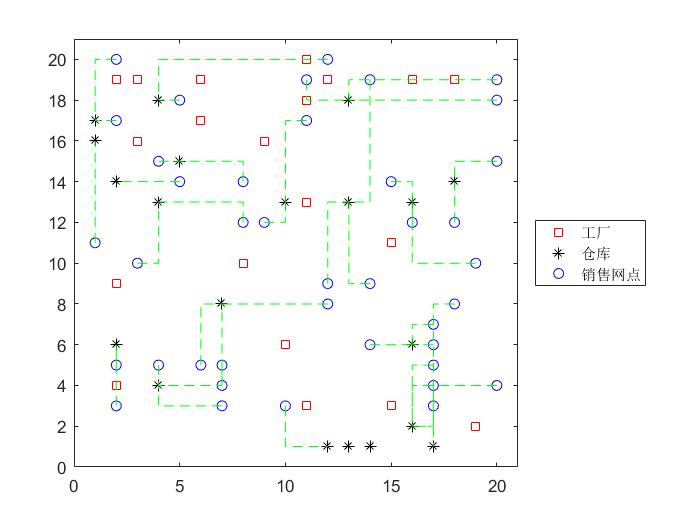
\includegraphics[width=8cm]{images/factory_location.jpg}
        \caption{工厂选址问题示意图}
        \label{fig:工厂选址问题示意图}
        \end{figure}
        % \textcolor[rgb]{1,0,0}{todo:图片:工厂选址问题示意图}
        \par
        假设我们已经知道各$f,w,s$的位置,并且假设有$p$种可销售的产品,$p$为第$p$种产品。设每个销售点$S$对产品$p$的销售量为$d(s,p)$,每个工厂$f$对产品$p$的产量不超过$pcap(f,p)$,仓库$w$的容量为$wcap(w)$,从仓库$w$转移到销售点$s$的产品$p$的量小于$turn(p)*wcap(p)$,其中$turn(p)$为产品转移率,并且假设每个销售点$s$只能有一个进货仓库。
        \par
        商品的转移费用依赖于$f,w,s$之间的距离,设$dist(a,b)$表示$ab$之间的距离,并且已知。则$a$到$b$转移产品$p$的花费为$dist(a,b)*tcost(p)$。其中:$tcost(p)$为产品单位距离的转移费用。\\
        设$pcost(f,p)$为工厂$f$生产单位产品$p$的费用。
        \par
        现在求工厂到仓库的产品转移量$x(p,f,w)$,使费用最小。并且求销售点$s$从哪个仓库进货使得费用最小($y(s,w)=1$表示$s$从$w$进货),则目标为
        \par
        目标1:$\text{运输量}\times(\text{成本费}+\text{运输费})$
        \begin{align*}
        obj1=\mathop{\sum}\limits_{f}\mathop{\sum}\limits_{p}\mathop{\sum}\limits_{w} x(p,f,w)\cdot (pcost(f,p)+tcost(p)\cdot dist(f,w))
        \end{align*}
        \par
        目标2:$\text{需求量} \times \text{运输费}$
        \begin{align*}
        obj2=\mathop{\sum}\limits_{s}\mathop{\sum}\limits_{w}\mathop{\sum}\limits_{p} d(s,p)\cdot tcost(p)\cdot dist(s,w)\cdot y(s,w)
        \end{align*}
        综合目标为
        \begin{align*}
        \mathop{\min}\limits_{xy} \ obj=obj1+obj2
        \end{align*}
        约束条件:\\
        \ding{172}工厂$f$的生产限制
        \begin{align*}
        \mathop{\sum}\limits_{w} x(p,f,w) \leqslant pcap(f,p)
        \end{align*}
        \ding{173}要满足需求量
        \begin{align*}
        \mathop{\sum}\limits_{f} x(p,f,w) = \mathop{\sum}\limits_{s} (d(s,p)\cdot y(s,w))
        \end{align*}
        \ding{174}仓库$W$的容量限制
        \begin{align*}
        \mathop{\sum}\limits_{p} \mathop{\sum}\limits_{s}(d(s,p) / turn(p))\cdot y(s,w) \leqslant wcap(w)
        \end{align*}
        \ding{175}每个$s$只能有一个进货仓库$w$
        \begin{align*}
        &\mathop{\sum}\limits_{w} y(s,w) = 1\\
        &x \geqslant 0\\
        &y \in \{0,1\}
        \end{align*}
        \par
        上述问题是一个混合线性规划问题,其求解程序如下
        \begin{lstlisting}[language = Matlab]
        %% 工厂,仓库和销售网点
        % 这个例子说明了如何建立和求解混合整数线性规划问题。
        % 问题是要找到一组工厂,仓库和销售网点之间的最佳生产和分销水平。
        %% 随机生成位置
        rng default % for reproducibility
        N = 20; % N from 10 to 30 seems to work. Choose large values with caution.
        N2 = N*N;
        f = 0.05; % 比重 of factories
        w = 0.05; % density of warehouses
        s = 0.1; % density of sales outlets
        F = floor(f*N2); % number of factories
        W = floor(w*N2); % number of warehouses
        S = floor(s*N2); % number of sales outlets
        xyloc = randperm(N2,F+W+S); % unique locations of facilities
        [xloc,yloc] = ind2sub([N N],xyloc);
        h = figure;
        plot(xloc(1:F),yloc(1:F),'rs',xloc(F+1:F+W),yloc(F+1:F+W),'k*',...
            xloc(F+W+1:F+W+S),yloc(F+W+1:F+W+S),'bo');
        legend('工厂','仓库','销售网点','Location','EastOutside')
        xlim([0 N+1]);ylim([0 N+1])

        %% 生成随机容量,成本,和需求
        P = 20; % 20种产品
        % 产品的生产成本在20到100之间
        pcost = 80*rand(F,P) + 20;%每个工厂F生产产品P的成本矩阵pcost
        % 产品生产的限量 between 500 and 1500 for each product/factory
        pcap = 1000*rand(F,P) + 500;%每个工厂F生产产品P的限量
        % 仓库容量限制 between P*400 and P*800 for each product/warehouse
        wcap = P*400*rand(W,P) + P*400;%每个仓库W存储产品P的限量
        % 产品转移率 between 1 and 3 for each product
        turn = 2*rand(1,P) + 1;%20个产品的转移率在1-3之间
        % 单位距离转移产品的花费 between 5 and 10 for each product
        tcost = 5*rand(1,P) + 5;
        % 销售点的产品需求 between 200 and 500 for each product/outlet
        d = 300*rand(S,P) + 200;
        %% 生成目标和约束矩阵和向量
        obj1 = zeros(P,F,W);
        obj2 = zeros(S,W);
        distfw = zeros(F,W); % 距离矩阵:工厂-仓库
        for ii = 1:F
            for jj = 1:W
                distfw(ii,jj) = abs(xloc(ii) - xloc(F + jj)) + abs(yloc(ii) - yloc(F + jj));
            end
        end
        distsw = zeros(S,W); % 距离矩阵:销售网点-仓库
        for ii = 1:S
            for jj = 1:W
                distsw(ii,jj) = abs(xloc(F + W + ii) - xloc(F + jj)) ...
                    + abs(yloc(F + W + ii) - yloc(F + jj));
            end
        end
        % 构建目标1和目标2 obj1 and obj2.
        for ii = 1:P
            for jj = 1:F
                for kk = 1:W
                    obj1(ii,jj,kk) = pcost(jj,ii) + tcost(ii)*distfw(jj,kk);
                end
            end
        end
        for ii = 1:S
            for jj = 1:W
                obj2(ii,jj) = distsw(ii,jj)*sum(d(ii,:).*tcost);
            end
        end
        % 合并目标
        obj = [obj1(:);obj2(:)]; % obj is the objective function vector
        matwid = length(obj);
        Aineq = spalloc(P*F + W,matwid,P*F*W + S*W); % 配置 sparse Aeq为非零元素配置内存
        bineq = zeros(P*F + W,1); % Allocate bineq as full
        % Zero matrices of convenient sizes:
        clearer1 = zeros(size(obj1));
        clearer12 = clearer1(:);
        clearer2 = zeros(size(obj2));
        clearer22 = clearer2(:);
        % 首先,工厂生产量的约束
        counter = 1;
        for ii = 1:F
            for jj = 1:P
                xtemp = clearer1;
                xtemp(jj,ii,:) = 1; % Sum over warehouses for each product and factory为每个产品和工厂仓库求和
                xtemp = sparse([xtemp(:);clearer22]); % Convert to sparse
                Aineq(counter,:) = xtemp'; % Fill in the row
                bineq(counter) = pcap(ii,jj);
                counter = counter + 1;
            end
        end
        % 然后,仓库容量约束
        vj = zeros(S,1); % The multipliers
        for jj = 1:S
            vj(jj) = sum(d(jj,:)./turn); % A sum of P elements
        end
        for ii = 1:W
            xtemp = clearer2;
            xtemp(:,ii) = vj;
            xtemp = sparse([clearer12;xtemp(:)]); % Convert to sparse
            Aineq(counter,:) = xtemp'; % Fill in the row
            bineq(counter) = wcap(ii);
            counter = counter + 1;
        end
        Aeq = spalloc(P*W + S,matwid,P*W*(F+S) + S*W); % Allocate as sparse
        beq = zeros(P*W + S,1); % Allocate vectors as full分配向量为满
        % 然后,需求满足
        counter = 1;
        for ii = 1:P
            for jj = 1:W
                xtemp = clearer1;
                xtemp(ii,:,jj) = 1;
                xtemp2 = clearer2;
                xtemp2(:,jj) = -d(:,ii);
                xtemp = sparse([xtemp(:);xtemp2(:)]'); % Change to sparse row
                Aeq(counter,:) = xtemp; % Fill in row
                counter = counter + 1;
            end
        end
        % 最终,每一个销售网点只有一个仓库对于
        for ii = 1:S
            xtemp = clearer2;
            xtemp(ii,:) = 1;
            xtemp = sparse([clearer12;xtemp(:)]'); % Change to sparse row改变稀疏的行
            Aeq(counter,:) = xtemp; % Fill in row
            beq(counter) = 1;
            counter = counter + 1;
        end
        %% 设置变量界限和整数变量
        intcon = P*F*W+1:length(obj);%整数变量
        lb = zeros(length(obj),1);
        ub = Inf(length(obj),1);
        ub(P*F*W+1:end) = 1;
        %% 求解问题
        opts = optimoptions('intlinprog','Display','off','PlotFcns',@optimplotmilp);
        [solution,fval,exitflag,output] = intlinprog(obj,intcon,...
                                             Aineq,bineq,Aeq,beq,lb,ub,opts);
        if isempty(solution) % 如果问题是不可行的,或者你提前停止没有解决方案
            disp('intlinprog did not return a solution.')
            return
        end
        %% 检查解决方案
        exitflag
        infeas1 = max(Aineq*solution - bineq)
        infeas2 = norm(Aeq*solution - beq,Inf)
        diffint = norm(solution(intcon) - round(solution(intcon)),Inf)
        solution(intcon) = round(solution(intcon));
        infeas1 = max(Aineq*solution - bineq)
        infeas2 = norm(Aeq*solution - beq,Inf)
        diffrounding = norm(fval - obj(:)'*solution,Inf)
        solution1 = solution(1:P*F*W); % The continuous variables
        solution2 = solution(intcon); % The integer variables
        solution1 = reshape(solution1,P,F,W);
        solution2 = reshape(solution2,S,W);
        outlets = sum(solution2,1) % Sum over the sales outlets
        figure(h);
        hold on
        for ii = 1:S
            jj = find(solution2(ii,:)); % Index of warehouse associated with ii
            xsales = xloc(F+W+ii); ysales = yloc(F+W+ii);
            xwarehouse = xloc(F+jj); ywarehouse = yloc(F+jj);
            if rand(1) < .5 % Draw y direction first half the time
                plot([xsales,xsales,xwarehouse],[ysales,ywarehouse,ywarehouse],'g--')
            else % Draw x direction first the rest of the time
                plot([xsales,xwarehouse,xwarehouse],[ysales,ysales,ywarehouse],'g--')
            end
        end
        hold off
        title('Mapping of sales outlets to warehouses')
        \end{lstlisting}
% \end{document}
